\documentclass[leqno]{article}
% Shared QBT/Soln pack preamble for resources.danieljsmith.org.
\usepackage{graphicx}
\usepackage{dsfont}
\usepackage{mathtools}
\usepackage{amssymb}
\usepackage{amsmath}
\usepackage{amsthm}
\usepackage{float}
\usepackage{ragged2e}
\usepackage{tensor}
\usepackage{fancyhdr}
\usepackage{empheq}
\usepackage[most]{tcolorbox}
\usepackage{enumitem}
\usepackage{dirtytalk}
\usepackage{marginnote}
\usepackage{microtype}
\usepackage[
  a4paper,
  left=0.8in,
  right=1in,
  top=1in,
  bottom=0.5in,
  headheight=14pt,
  headsep=0.4in
]{geometry}
\setlength{\parindent}{0cm}

% TikZ / PGFPlots
\usepackage{pgfplots}
\pgfplotsset{compat=1.18}
\usepgfplotslibrary{fillbetween, polar}
\usetikzlibrary{calc, positioning}
\usetikzlibrary{angles, quotes}
\usetikzlibrary{arrows.meta}
\usetikzlibrary{decorations.pathreplacing, decorations.markings}
\usetikzlibrary{patterns}
\usetikzlibrary{intersections}

% Links and contents
\usepackage[colorlinks=true,linkcolor=black,citecolor=magenta,urlcolor=black]{hyperref}%
\urlstyle{same}

% Pack macros
\RenewDocumentCommand{\marks}{o m}{%
  \IfValueTF{#1}%
    {\marginnote{\raggedright\textbf{[#2]}}[#1]}%
    {\marginnote{\raggedright\textbf{[#2]}}}%
}

\newcommand{\vspacerule}[2]{%
  \par\vspace*{#1}%
  \noindent\hrulefill\par
  \vspace*{#2}%
}

\definecolor{scarlet}{RGB}{205, 40, 75}

% Worked-solution box, adapted from the TMUA worked-solutions box. A white breakable box with a left scarlet rule and no surrounding
% frame or tint. A part that breaks fills the rest of its page, so the rule
% runs to the bottom margin; the unbroken or last part ends in a short
% horizontal foot rule so a solution visibly stops. Unlike the TMUA box there
% is no answer label and no extra \parskip: these solutions mix \\ line breaks
% with blank lines, so paragraph skips would make the spacing uneven. The box
% does not grow to the left, so the rule sits at the text edge; growing to the
% right keeps the usable line width close to the old tcolorbox Solution box.
\newtcolorbox{djsSolution}{%
  enhanced, breakable, frame hidden, sharp corners, colback=white,
  height fixed for=first and middle, height fill,
  extras unbroken and last={natural height},
  borderline west={2.2pt}{0pt}{scarlet},
  left=11pt, right=0pt, top=5pt, bottom=13pt,
  before skip=13pt, after skip=4pt,
  grow to right by=10mm,
  overlay unbroken and last={%
    \fill[scarlet] (frame.south west)
      rectangle ([xshift=3.5cm, yshift=2.2pt]frame.south west);},
  before upper={{\color{scarlet}\bfseries Solution}\par\vspace{4pt}}}

% Optional smaller figure inside a solution box. \scalebox shrinks node text
% with the drawing. Not applied to existing figures.
\newcommand{\SolnFigureScale}{0.85}
\newsavebox{\djsSolnFigureBox}
\newenvironment{djsSolutionFigure}
  {\par\vspace{4pt}\begin{center}\begin{lrbox}{\djsSolnFigureBox}}
  {\end{lrbox}\scalebox{\SolnFigureScale}{\usebox{\djsSolnFigureBox}}%
   \end{center}\vspace{2pt}\par}

\newcommand{\cxl}[2]{%
  \tikz[baseline=(X.base)]{%
    \node[inner sep=0pt, outer sep=0pt, text=#1] (X) {$#2$};
    \draw[#1, line width=0.4pt] (X.south west)--(X.north east);
  }%
}

% Page-style hook run at the contents page and each question's opening page.
% A no-op for QBT packs; \djsSolnHeader points it at the fancy header.
\newcommand{\djsQuestionPageStyle}{}

\newcommand{\questionitem}{%
  \djsQuestionPageStyle
  \item\phantomsection
  \addcontentsline{toc}{section}{Question \number\value{enumi}}%
}

\renewcommand{\contentsname}{Questions}

\newcommand{\djsPackHeader}[1]{%
  \pagestyle{fancy}%
  \fancyhead{}%
  \fancyfoot{}%
  \renewcommand{\headrulewidth}{0.9pt}%
  \lhead{#1}%
  \chead{}%
  \rhead{\href{https://danieljsmith.org}{danieljsmith.org}}%
}

\newcommand{\djsQbtHeader}[1]{%
  \djsPackHeader{#1}%
}

% Solutions packs show the header only on the contents page and each
% question's opening page, so it never appears part-way through a solution.
% \thispagestyle marks the next page shipped out, which is the question's
% page because every solution question starts after a \newpage.
\newcommand{\djsSolnHeader}[1]{%
  \djsPackHeader{\textit{Solutions} - #1}%
  \pagestyle{empty}%
  \renewcommand{\djsQuestionPageStyle}{\thispagestyle{fancy}}%
}

\newcommand{\djsFrontMatter}{%
  \djsQuestionPageStyle
  \vspace*{20pt}%
  \tableofcontents
  \newpage
}


\djsSolnHeader{Centre of Mass of Systems of Particles}

\begin{document}
\djsFrontMatter
\begin{enumerate}[
  label=\textbf{\arabic*.},
  leftmargin=*,
  topsep=0pt,
  partopsep=0pt,
  parsep=0pt
]

% ---- Question 1 ----
\questionitem
% [Source: _QBT___Solns__Centre_of_Mass_of_Systems_of_Particles, Q1]

Three particles of masses $m$, $2m$ and $km$ are placed at the points $A(a,0)$, $B(-2a,3a)$ and $C(2a,-a)$ respectively, where $k>0$. \\

The centre of mass of the three particles is the point with coordinates $(\bar{x}, \bar{y})$. \\

\begin{enumerate}[label=\textbf{(\alph*)}]
  \item
  \begin{enumerate}[label=(\roman*)]
    \item Find $\bar{x}$ in terms of $a$ and $k$.
    \item Find $\bar{y}$ in terms of $a$ and $k$.
  \end{enumerate}
  \marks{4} 
  \item Given that the centre of mass lies on the circle with centre $(a,0)$ and radius $\dfrac{\sqrt{2}}{2}a$, find the possible values of $k$. \marks{2} 
\end{enumerate}

\vspace*{10pt}

\begin{tcolorbox}[colback=white, colframe=scarlet, title={\textbf{Solution}}, breakable, grow to left by=6mm, grow to right by=10mm]
\begin{enumerate}[label=\textbf{(\alph*)}, start=1]
  \item The total mass is
  \[
  M=m+2m+km=(k+3)m
  \]
  \begin{enumerate}[label=\textbf{(\roman*)}, start=1]
    \item Using the formula for the $x$-coordinate of the centre of mass,
    \[
    M\bar{x}=m(a)+2m(-2a)+km(2a)
    \]
    So
    \begin{align*}
    (k+3)m\bar{x} &= am-4am+2kam \\
    &= am(2k-3)
    \end{align*}
    Hence
    \[
    \bar{x}=\frac{a(2k-3)}{k+3}
    \]
    So the $x$-coordinate is $\displaystyle \bar{x}=\frac{a(2k-3)}{k+3}$.

    \item Using the formula for the $y$-coordinate of the centre of mass,
    \[
    M\bar{y}=m(0)+2m(3a)+km(-a)
    \]
    So
    \begin{align*}
    (k+3)m\bar{y} &= 0+6am-kam \\
    &= am(6-k)
    \end{align*}
    Hence
    \[
    \bar{y}=\frac{a(6-k)}{k+3}
    \]
    So the $y$-coordinate is $\displaystyle \bar{y}=\frac{a(6-k)}{k+3}$.
  \end{enumerate}

  \item Since the centre of mass lies on the circle with centre $(a,0)$ and radius $\dfrac{\sqrt{2}}{2}a$,
  \[
  (\bar{x}-a)^2+\bar{y}^2=\left(\frac{\sqrt{2}}{2}a\right)^2=\frac{a^2}{2}
  \]
  From part (a),
  \begin{align*}
  \bar{x}-a &= \frac{a(2k-3)}{k+3}-a \\
  &= a\left(\frac{2k-3-(k+3)}{k+3}\right) \\
  &= \frac{a(k-6)}{k+3}
  \end{align*}
  and
  \[
  \bar{y}=\frac{a(6-k)}{k+3}=-\frac{a(k-6)}{k+3}
  \]
  Substituting into the circle equation,
  \begin{align*}
  \left(\frac{a(k-6)}{k+3}\right)^2+\left(-\frac{a(k-6)}{k+3}\right)^2 &= \frac{a^2}{2} \\
  2\left(\frac{a(k-6)}{k+3}\right)^2 &= \frac{a^2}{2}
  \end{align*}
  So
  \[
  4(k-6)^2=(k+3)^2
  \]
  Expanding,
  \begin{align*}
  4(k^2-12k+36) &= k^2+6k+9 \\
  4k^2-48k+144 &= k^2+6k+9 \\
  3k^2-54k+135 &= 0 \\
  k^2-18k+45 &= 0
  \end{align*}
  Factorising,
  \[
  (k-3)(k-15)=0
  \]
  Hence the possible values of $k$ are
  \[
  k=3 \quad \text{or} \quad k=15
  \]
\end{enumerate}
\end{tcolorbox}


\newpage

% ---- Question 2 ----
\questionitem
% [Source: _QBT___Solns__Centre_of_Mass_of_Systems_of_Particles, Q2]

\begin{figure}[H]
    \centering
\begin{tikzpicture}[x=4cm,y=4cm]
\coordinate (O) at (0,0);
\coordinate (A) at (2,0);
\coordinate (B) at (2,1);
\coordinate (C) at (0,1);
\coordinate (Xend) at (2.55,0);
\coordinate (Yend) at (0,1.35);

\draw[-{Stealth[length=3mm]}, thick] (-0.04,0) -- (Xend);
\draw[-{Stealth[length=3mm]}, thick] (0,-0.04) -- (Yend);
\draw[thick] (O) -- (A) -- (B) -- (C) -- cycle;

\node[below left] at (O) {$O$};
\node[below right] at (A) {$A\,(2,0)$};
\node[above right] at (B) {$B\,(2,1)$};
\node[above right] at (C) {$C\,(0,1)$};
\node[right] at (Xend) {$x$};
\node[above] at (Yend) {$y$};
\end{tikzpicture}
\end{figure}


The diagram shows a light rectangular lamina $OABC$ where $O$ is the origin of the coordinate system in which the points $A$, $B$ and $C$ have coordinates $(2, 0)$, $(2, 1)$ and $(0, 1)$ respectively. Coordinates refer to the axes shown and the units are metres. \\

The following three forces are applied to the lamina. 

\begin{align*}
&\begin{pmatrix}
p \\
2q
\end{pmatrix}\,\mathrm{N} \text{ at the point } (1, 0) \\[1em]
&\begin{pmatrix}
-q \\
p
\end{pmatrix}\,\mathrm{N} \text{ at the point } C \\[1em]
&\begin{pmatrix}
-3 \\
-6
\end{pmatrix}\,\mathrm{N} \text{ at the point } (t, 1), \text{ where } 0 \le t \le 2 \\
\end{align*}

The three forces form a couple of magnitude $3\,\mathrm{N\,m}$ in the anticlockwise direction. \\

\begin{enumerate}[label=\textbf{(\alph*)}]
  \item Determine the values of $p$, $q$ and $t$. \marks{5} \\
\end{enumerate}

The three forces are removed. The lamina is in the same position as shown in the diagram. \\

Three particles are now attached to certain points on the lamina as follows. \\

\begin{enumerate}[label=\textbf{(\alph*)}, resume]
  \item Find the coordinates of the composite body's centre of mass. Give your answer in terms of $\lambda$, where the particles are
  \begin{itemize}
    \item a particle of mass $2\,\mathrm{kg}$ at the point $(2\lambda^2, \lambda)$, where $0 \le \lambda \le 1$
    \item a particle of mass $1\,\mathrm{kg}$ at the point $A$
    \item a particle of mass $1\,\mathrm{kg}$ at the point $C$
  \end{itemize}
  \marks{3} 
  \item Show that, as $\lambda$ varies, the centre of mass of the combined object lies on the curve
  \[
  x = 4y^2 - 2y + k
  \]
  where $k$ is a constant to be determined. \marks{3} \\
\end{enumerate}

\vspace*{20pt}

\begin{tcolorbox}[colback=white, colframe=scarlet, title={\textbf{Solution}}, breakable, grow to left by=6mm, grow to right by=10mm]
\begin{enumerate}[label=\textbf{(\alph*)}, start=1]
  \item Since the three forces form a couple, their resultant force is zero.

  Resolving in the $x$- and $y$-directions:
  \[
  p-q-3=0,
  \qquad
  p+2q-6=0
  \]
  Subtracting the first equation from the second gives
  \[
  3q-3=0
  \]
  so
  \[
  q=1.
  \]
  Substituting into $p-q-3=0$:
  \[
  p-1-3=0 \implies p=4.
  \]

  Now take moments about $O$, with anticlockwise positive.

  For a force $(F_x,F_y)$ acting at $(x,y)$, the moment about $O$ is
  \[
  xF_y-yF_x.
  \]

  So the moments of the three forces are
  \begin{align*}
  M_1 &= 1(2q)-0(p)=2q, \\
  M_2 &= 0(p)-1(-q)=q, \\
  M_3 &= t(-6)-1(-3)=3-6t.
  \end{align*}

  Since the forces form an anticlockwise couple of magnitude $3\,\mathrm{N\,m}$,
  \[
  M_1+M_2+M_3=3.
  \]
  Hence
  \[
  2q+q+3-6t=3.
  \]
  Using $q=1$:
  \[
  2+1+3-6t=3.
  \]
  Therefore
  \[
  6-6t=3 \implies 6t=3 \implies t=\frac12.
  \]

  So
  \[
  p=4, \qquad q=1, \qquad t=\frac12.
  \]

  \item The lamina is light, so its mass is taken to be zero.

  Let the centre of mass of the composite body be $(x,y)$.

  The total mass is
  \[
  2+1+1=4.
  \]

  Using $Mx=M_1x_1+M_2x_2+M_3x_3$,
  \[
  4x=2(2\lambda^2)+1(2)+1(0)=4\lambda^2+2.
  \]
  So
  \[
  x=\lambda^2+\frac12.
  \]

  Using $My=M_1y_1+M_2y_2+M_3y_3$,
  \[
  4y=2(\lambda)+1(0)+1(1)=2\lambda+1.
  \]
  So
  \[
  y=\frac{2\lambda+1}{4}.
  \]

  Hence the centre of mass is
  \[
  \left(\lambda^2+\frac12,\,\frac{2\lambda+1}{4}\right).
  \]

  \item From part (b), the centre of mass has coordinates
  \[
  x=\lambda^2+\frac12,
  \qquad
  y=\frac{2\lambda+1}{4}.
  \]

  Rearranging the expression for $y$,
  \[
  4y=2\lambda+1
  \]
  so
  \[
  \lambda=\frac{4y-1}{2}.
  \]

  Substitute this into the expression for $x$:
  \begin{align*}
  x&=\left(\frac{4y-1}{2}\right)^2+\frac12 \\
   &=\frac{16y^2-8y+1}{4}+\frac12 \\
   &=4y^2-2y+\frac14+\frac12 \\
   &=4y^2-2y+\frac34.
  \end{align*}

  Therefore the locus is
  \[
  x=4y^2-2y+k
  \]
  with
  \[
  k=\frac34.
  \]
\end{enumerate}
\end{tcolorbox}


\newpage

% ---- Question 3 ----
\questionitem
% [Source: _QBT___Solns__Centre_of_Mass_of_Systems_of_Particles, Q3]

Three particles of masses $2m$, $5m$ and $3m$ are placed at the points $(1, -4)$, $(-3, 2)$ and $(q, 2q - 1)$ respectively. \\

The value of $q$ is such that the distance of the centre of mass of the three particles from the point $(1, 0)$ is as small as possible. \\

Find the value of $q$. \marks{7} \\

\vspace*{10pt}

\begin{tcolorbox}[colback=white, colframe=scarlet, title={\textbf{Solution}}, breakable, grow to left by=6mm, grow to right by=10mm]
Let the centre of mass be \(G(\bar x,\bar y)\).

The total mass is
\[
2m+5m+3m=10m
\]

Using the centre of mass formula for the coordinates,
\[
10m\bar x=2m(1)+5m(-3)+3m(q)
\]
so
\begin{align*}
10\bar x&=2-15+3q\\
\bar x&=\frac{3q-13}{10}
\end{align*}

Also,
\[
10m\bar y=2m(-4)+5m(2)+3m(2q-1)
\]
so
\begin{align*}
10\bar y&=-8+10+6q-3\\
&=6q-1\\
\bar y&=\frac{6q-1}{10}
\end{align*}

Hence
\[
G\left(\frac{3q-13}{10},\frac{6q-1}{10}\right)
\]

Let the distance from \(G\) to \((1,0)\) be \(d\). Then
\begin{align*}
d^2&=\left(\frac{3q-13}{10}-1\right)^2+\left(\frac{6q-1}{10}\right)^2\\
&=\left(\frac{3q-23}{10}\right)^2+\left(\frac{6q-1}{10}\right)^2\\
&=\frac{(3q-23)^2+(6q-1)^2}{100}
\end{align*}

Now expand:
\begin{align*}
(3q-23)^2+(6q-1)^2&=9q^2-138q+529+36q^2-12q+1\\
&=45q^2-150q+530
\end{align*}

So
\[
d^2=\frac{45q^2-150q+530}{100}
\]

To make \(d\) as small as possible, it is enough to make \(d^2\) as small as possible. Complete the square:
\begin{align*}
45q^2-150q+530
&=45\left(q^2-\frac{10}{3}q\right)+530\\
&=45\left[\left(q-\frac{5}{3}\right)^2-\frac{25}{9}\right]+530\\
&=45\left(q-\frac{5}{3}\right)^2-125+530\\
&=45\left(q-\frac{5}{3}\right)^2+405
\end{align*}

Since \(45\left(q-\frac{5}{3}\right)^2\ge 0\), this expression is smallest when
\[
q-\frac{5}{3}=0
\]

Therefore,
\[
q=\frac{5}{3}
\]
\end{tcolorbox}


\newpage

% ---- Question 4 ----
\questionitem
% [Source: _QBT___Solns__Centre_of_Mass_of_Systems_of_Particles, Q4]

\begin{figure}[H]
    \centering
\begin{tikzpicture}[scale=0.7]
\def\cx{1}
\def\cy{-1}
\def\r{5}

\coordinate (O) at (0,0);
\coordinate (A) at (5,0);
\coordinate (B) at (-2,1);
\coordinate (C) at (3,-4);
\coordinate (D) at (0,-3);

\draw[-{Stealth[length=3mm]}, thick] (-6,0) -- (8,0) node[right] {$x$};
\draw[-{Stealth[length=3mm]}, thick] (0,-7) -- (0,6) node[above] {$y$};
\draw[thick] (\cx,\cy) circle (\r);

\fill[black] (A) circle (3pt);
\node[below right] at (A) {$A$};

\fill[black] (B) circle (3pt);
\node[above left] at (B) {$B$};

\fill[black] (C) circle (3pt);
\node[below right] at (C) {$C$};

\fill[black] (D) circle (3pt);
\node[left] at (D) {$D$};

\node[above right] at (O) {$O$};
\end{tikzpicture}
\end{figure}


Four sensors are attached to a circular plate. \\

The plate is to be modelled as a uniform lamina and the four sensors as four particles. \\

The diagram shows the lamina, the four particles $A$, $B$, $C$ and $D$, and the coordinate axes. \\

The lamina has mass $6\,\mathrm{kg}$ and its centre of mass is at the point $(1,-1)$. \\

Particle $A$ has mass $4\,\mathrm{kg}$ and is at the point $(5,0)$. \\
Particle $B$ has mass $3\,\mathrm{kg}$ and is at the point $(-2,1)$. \\
Particle $C$ has mass $5\,\mathrm{kg}$ and is at the point $(3,-4)$. \\
Particle $D$ has mass $2\,\mathrm{kg}$ and is at the point $(0,-3)$. \\

Find the coordinates of the centre of mass of the system of plate and sensors. \marks{5} \\

\vspace*{10pt}

\begin{tcolorbox}[colback=white, colframe=scarlet, title={\textbf{Solution}}, breakable, grow to left by=6mm, grow to right by=10mm]
Treat the uniform lamina as a particle of mass $6\,\mathrm{kg}$ acting at its centre of mass $(1,-1)$.

Let the centre of mass of the whole system be $(\bar{x},\bar{y})$.

The total mass is
\[
M=6+4+3+5+2=20\,\mathrm{kg}
\]

For the $x$-coordinate, use the weighted average
\[
M\bar{x}=m_1x_1+m_2x_2+m_3x_3+m_4x_4+m_5x_5
\]
so
\begin{align*}
20\bar{x}
&=6(1)+4(5)+3(-2)+5(3)+2(0)\\
&=6+20-6+15+0\\
&=35
\end{align*}
Hence
\[
\bar{x}=\frac{35}{20}=\frac{7}{4}
\]

For the $y$-coordinate,
\[
M\bar{y}=m_1y_1+m_2y_2+m_3y_3+m_4y_4+m_5y_5
\]
so
\begin{align*}
20\bar{y}
&=6(-1)+4(0)+3(1)+5(-4)+2(-3)\\
&=-6+0+3-20-6\\
&=-29
\end{align*}
Hence
\[
\bar{y}=\frac{-29}{20}
\]

Therefore the centre of mass of the system is
\[
\left(\frac{7}{4},-\frac{29}{20}\right)
\]
In decimal form, this is $(1.75,-1.45)$.
\end{tcolorbox}


\newpage

% ---- Question 5 ----
\questionitem
% [Source: _QBT___Solns__Centre_of_Mass_of_Systems_of_Particles, Q5]

\begin{figure}[H]
    \centering
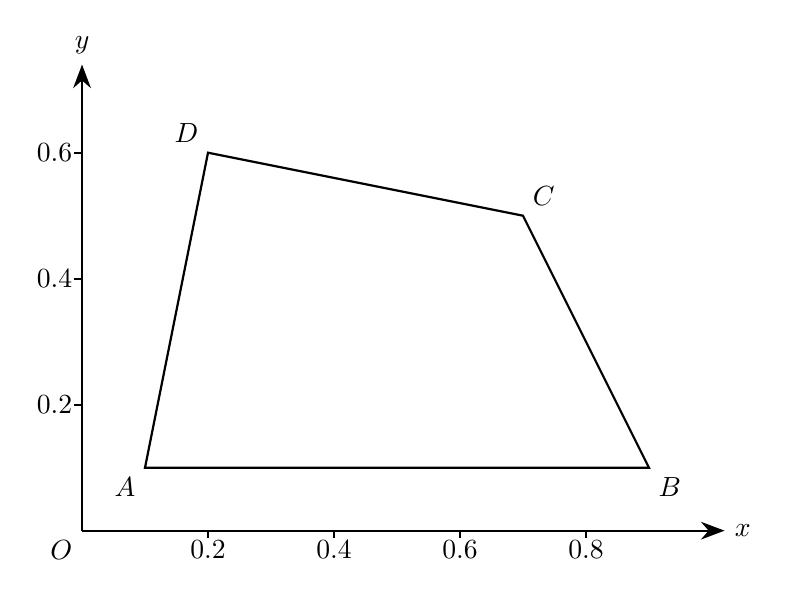
\begin{tikzpicture}[x=8cm,y=8cm]
\def\xA{0.1}
\def\yA{0.1}
\def\xB{0.9}
\def\yB{0.1}
\def\xC{0.7}
\def\yC{0.5}
\def\xD{0.2}
\def\yD{0.6}
\coordinate (O) at (0,0);
\coordinate (A) at (\xA,\yA);
\coordinate (B) at (\xB,\yB);
\coordinate (C) at (\xC,\yC);
\coordinate (D) at (\xD,\yD);
\coordinate (Xend) at (1.02,0);
\coordinate (Yend) at (0,0.74);

\draw[-{Stealth[length=3mm]}, thick] (O) -- (Xend) node[right] {$x$};
\draw[-{Stealth[length=3mm]}, thick] (O) -- (Yend) node[above] {$y$};

\foreach \tick/\lbl in {0.2/0.2,0.4/0.4,0.6/0.6,0.8/0.8} {
  \draw[thick] (\tick,0) -- ++(0,-0.012);
  \node[below] at (\tick,0) {$\lbl$};
}
\foreach \tick/\lbl in {0.2/0.2,0.4/0.4,0.6/0.6} {
  \draw[thick] (0,\tick) -- ++(-0.012,0);
  \node[left] at (0,\tick) {$\lbl$};
}

\draw[thick] (A) -- (B) -- (C) -- (D) -- cycle;

\node[below left] at (O) {$O$};
\node[below left] at (A) {$A$};
\node[below right] at (B) {$B$};
\node[above right] at (C) {$C$};
\node[above left] at (D) {$D$};


\end{tikzpicture}
\end{figure}


Particles $A$, $B$, $C$ and $D$ of masses $1\,\mathrm{kg}$, $2\,\mathrm{kg}$, $3\,\mathrm{kg}$ and $4\,\mathrm{kg}$ respectively are joined by light rigid rods to form the quadrilateral frame shown in the diagram. The particles are at the points $A(0.1,0.1)$, $B(0.9,0.1)$, $C(0.7,0.5)$ and $D(0.2,0.6)$, where coordinates are measured in metres. \\

$G$, the centre of mass of the frame, has coordinates $(\bar{x},\bar{y})$. \\

\begin{enumerate}[label=\textbf{(\alph*)}]
  \item Show that $\bar{y}=0.42$. Find $\bar{x}$. \marks{3} \\
  \item Using your answer to part (a), explain why the frame cannot be in equilibrium in a horizontal plane if it is supported by a single peg touching the frame at one point. \marks{1} \\
\end{enumerate}

\vspace*{10pt}

\begin{tcolorbox}[colback=white, colframe=scarlet, title={\textbf{Solution}}, breakable, grow to left by=6mm, grow to right by=10mm]
\begin{enumerate}[label=\textbf{(\alph*)}, start=1]
  \item The total mass of the frame is
  \[
  M=1+2+3+4=10
  \]

  Using the centre of mass formula for particles,
  \[
  M\bar{x}=\sum mx, \qquad M\bar{y}=\sum my
  \]

  For the \(y\)-coordinate,
  \[
  10\bar{y}=1(0.1)+2(0.1)+3(0.5)+4(0.6)
  \]
  \[
  10\bar{y}=0.1+0.2+1.5+2.4=4.2
  \]
  \[
  \bar{y}=\frac{4.2}{10}=0.42
  \]

  So \(\bar{y}=0.42\), as required.

  For the \(x\)-coordinate,
  \[
  10\bar{x}=1(0.1)+2(0.9)+3(0.7)+4(0.2)
  \]
  \[
  10\bar{x}=0.1+1.8+2.1+0.8=4.8
  \]
  \[
  \bar{x}=\frac{4.8}{10}=0.48
  \]

  Hence the centre of mass is
  \[
  G=(\bar{x},\bar{y})=(0.48,0.42)
  \]

  \item For equilibrium on a single peg, the peg must be vertically below the centre of mass.

  So in the horizontal plane, the peg would have to touch the frame at \(G=(0.48,0.42)\).

  But this point is not on the frame itself; it lies inside the quadrilateral, not on any of its sides.

  Therefore the frame cannot be in equilibrium if it is supported by a single peg touching the frame at one point.
\end{enumerate}
\end{tcolorbox}


\newpage

% ---- Question 6 ----
\questionitem
% [Source: _QBT___Solns__Centre_of_Mass_of_Systems_of_Particles, Q6]

Four particles of mass $m$, $2m$, $4m$ and $\lambda m$ are placed at points with coordinates $(0,0)$, $(2,3)$, $(1,-1)$ and $(4,2)$ respectively. The centre of mass of the system is at $(2,k)$. \\

\begin{enumerate}[label=\textbf{(\alph*)}]
  \item Show that $\lambda = 3$. \marks{4} \\
  \item Calculate the value of $k$. \marks{3} \\
\end{enumerate}

\vspace*{10pt}

\begin{tcolorbox}[colback=white, colframe=scarlet, title={\textbf{Solution}}, breakable, grow to left by=6mm, grow to right by=10mm]
\begin{enumerate}[label=\textbf{(\alph*)}, start=1]
  \item Let the total mass be \(M\). Then
\[
M=m+2m+4m+\lambda m=(7+\lambda)m
\]
Using the \(x\)-coordinate of the centre of mass, with centre \((2,k)\),
\[
M\cdot 2=m\cdot 0+2m\cdot 2+4m\cdot 1+\lambda m\cdot 4
\]
So
\begin{align*}
2(7+\lambda)m&=0+4m+4m+4\lambda m\\
2(7+\lambda)&=8+4\lambda\\
14+2\lambda&=8+4\lambda\\
6&=2\lambda\\
\lambda&=3
\end{align*}
Hence \(\lambda=3\).

  \item Now use the \(y\)-coordinate of the centre of mass. Since \(\lambda=3\),
\[
M=(7+3)m=10m
\]
Also,
\[
M\cdot k=m\cdot 0+2m\cdot 3+4m\cdot(-1)+3m\cdot 2
\]
So
\begin{align*}
10mk&=0+6m-4m+6m\\
10mk&=8m\\
k&=\frac{8}{10}\\
k&=\frac45
\end{align*}
So the value of \(k\) is \(\frac45\).
\end{enumerate}
\end{tcolorbox}


\newpage

% ---- Question 7 ----
\questionitem
% [Source: _QBT___Solns__Centre_of_Mass_of_Systems_of_Particles, Q7]

\begin{figure}[H]
    \centering
\begin{tikzpicture}[x=0.7cm,y=0.7cm]
\def\xmax{12}
\def\ymax{11}
\pgfmathsetmacro{\xint}{3/2}
\pgfmathsetmacro{\xtop}{(\ymax+3)/2}
\coordinate (O) at (0,0);
\coordinate (X) at (\xmax,0);
\coordinate (Y) at (0,\ymax);
\coordinate (A) at (1,9);
\coordinate (B) at (4,2);
\coordinate (C) at (10,7);
\coordinate (D) at (2,5);
\coordinate (L1) at (\xint,0);
\coordinate (L2) at (\xtop,\ymax);

\draw[-{Stealth[length=3mm]}, thick] (O) -- (X) node[right] {$x$};
\draw[-{Stealth[length=3mm]}, thick] (O) -- (Y) node[above] {$y$};
\draw[dashed, thick] (L1) -- (L2);
\node[right] at ($(L1)!0.9!(L2)$) {$y=2x-3$};

\fill[black] (A) circle (2pt);
\fill[black] (B) circle (2pt);
\fill[black] (C) circle (2pt);
\fill[black] (D) circle (2pt);

\node[below left] at (O) {$O$};
\node[above left] at (A) {$A$};
\node[below right] at (B) {$B$};
\node[above right] at (C) {$C$};
\node[below left] at (D) {$D$};
\end{tikzpicture}
\end{figure}


The diagram shows four particles, $A$, $B$, $C$ and $D$, fixed in a horizontal plane which contains the $x$- and $y$-axes. \\

Particle $A$ has mass $3\,\mathrm{kg}$ and is attached at the point $(1, 9)$. \\
Particle $B$ has mass $4\,\mathrm{kg}$ and is attached at the point $(4, 2)$. \\
Particle $C$ has mass $5\,\mathrm{kg}$ and is attached at the point $(10, 7)$. \\
Particle $D$ has mass $m\,\mathrm{kg}$ and is attached at the point $(2, 5)$. \\

The centre of mass of the four particles lies on the line $y = 2x - 3$. \\
Find the value of $m$ and the coordinates of the centre of mass. \marks{6} \\

\vspace*{10pt}

\begin{tcolorbox}[colback=white, colframe=scarlet, title={\textbf{Solution}}, breakable, grow to left by=6mm, grow to right by=10mm]
Let the centre of mass be \((\bar{x},\bar{y})\).

The total mass is
\[
M=3+4+5+m=12+m
\]

Using the centre of mass formula for coordinates,
\[
M\bar{x}=3(1)+4(4)+5(10)+m(2)
\]
so
\begin{align*}
(12+m)\bar{x}&=3+16+50+2m\\
&=69+2m
\end{align*}
Hence
\[
\bar{x}=\frac{69+2m}{12+m}
\]

Similarly,
\[
M\bar{y}=3(9)+4(2)+5(7)+m(5)
\]
so
\begin{align*}
(12+m)\bar{y}&=27+8+35+5m\\
&=70+5m
\end{align*}
Hence
\[
\bar{y}=\frac{70+5m}{12+m}
\]

Since the centre of mass lies on the line \(y=2x-3\),
\[
\frac{70+5m}{12+m}=2\left(\frac{69+2m}{12+m}\right)-3
\]

Multiply through by \(12+m\):
\begin{align*}
70+5m&=2(69+2m)-3(12+m)\\
&=138+4m-36-3m\\
&=102+m
\end{align*}
Therefore
\begin{align*}
70+5m&=102+m\\
4m&=32\\
m&=8
\end{align*}

Now substitute \(m=8\).
Then the total mass is
\[
12+8=20
\]

So
\begin{align*}
\bar{x}&=\frac{69+2(8)}{20}=\frac{85}{20}=\frac{17}{4}\\
\bar{y}&=\frac{70+5(8)}{20}=\frac{110}{20}=\frac{11}{2}
\end{align*}

Therefore,
\[
m=8
\]
and the centre of mass is
\[
\left(\frac{17}{4},\frac{11}{2}\right)
\]
\end{tcolorbox}


\newpage

% ---- Question 8 ----
\questionitem
% [Source: _QBT___Solns__Centre_of_Mass_of_Systems_of_Particles, Q8]

\begin{figure}[H]
    \centering
\begin{tikzpicture}[scale=1.1]
\coordinate (O) at (0,0);
\coordinate (P) at (-1,3);
\coordinate (Q) at (1,-1);
\coordinate (R) at (4,2);
\coordinate (S) at (6,-2);

\foreach \x in {-2,-1,1,2,3,4,5,6,7} {
  \draw[dotted] (\x,-3) -- (\x,4);
}
\foreach \y in {-3,-2,-1,1,2,3,4} {
  \draw[dotted] (-2,\y) -- (7,\y);
}

\draw[-{Stealth[length=3mm]}, thick] (-2.4,0) -- (7.6,0) node[right] {$x$};
\draw[-{Stealth[length=3mm]}, thick] (0,-3.4) -- (0,4.6) node[above] {$y$};

\foreach \x/\lbl in {-2/-2,2/2,4/4,6/6} {
  \draw[thick] (\x,0.08) -- (\x,-0.08);
  \node[below] at (\x,0) {$\lbl$};
}
\foreach \y/\lbl in {-2/-2,2/2,4/4} {
  \draw[thick] (0.08,\y) -- (-0.08,\y);
  \node[left] at (0,\y) {$\lbl$};
}
\node[below left] at (O) {$O$};

\fill[black] (P) circle (1.5pt);
\fill[black] (Q) circle (1.5pt);
\fill[black] (R) circle (1.5pt);
\fill[black] (S) circle (1.5pt);

\node[left=2pt] at (P) {$P$};
\node[right=2pt] at (P) {$2m$};
\node[left=2pt] at (Q) {$Q$};
\node[right=2pt] at (Q) {$4m$};
\node[left=2pt] at (R) {$R$};
\node[right=2pt] at (R) {$3m$};
\node[left=2pt] at (S) {$S$};
\node[right=2pt] at (S) {$m$};
\end{tikzpicture}
\end{figure}


The diagram shows a system of four particles of masses $2m$, $4m$, $3m$ and $m$ situated in the $x$-$y$ plane at the points $P(-1,3)$, $Q(1,-1)$, $R(4,2)$ and $S(6,-2)$ respectively. \\

Find the coordinates of the centre of mass of the system. \marks{5} \\

\vspace*{10pt}

\begin{tcolorbox}[colback=white, colframe=scarlet, title={\textbf{Solution}}, breakable, grow to left by=6mm, grow to right by=10mm]
Let the centre of mass be \((\bar x,\bar y)\).

First find the total mass:
\[
M=2m+4m+3m+m=10m
\]

For the \(x\)-coordinate of the centre of mass, use the weighted average:
\[
M\bar x=2m(-1)+4m(1)+3m(4)+m(6)
\]
So
\[
10m\bar x=-2m+4m+12m+6m=20m
\]
Hence
\[
\bar x=2
\]

For the \(y\)-coordinate of the centre of mass:
\[
M\bar y=2m(3)+4m(-1)+3m(2)+m(-2)
\]
So
\[
10m\bar y=6m-4m+6m-2m=6m
\]
Hence
\[
\bar y=\frac{3}{5}
\]

Therefore the coordinates of the centre of mass are \((2,\tfrac{3}{5})\).
\end{tcolorbox}


\newpage

% ---- Question 9 ----
\questionitem
% [Source: _QBT___Solns__Centre_of_Mass_of_Systems_of_Particles, Q9]

Four particles of masses $m$, $2m$, $3m$ and $km$ are positioned at the points with coordinates $(-a, a)$, $(2a, -2a)$, $(0, 0)$ and $(\mu a, 2\mu a)$ respectively, where $k$ and $\mu$ are constants. \\

The centre of mass of the four particles is at the point with coordinates $(2a, 3a)$. \\

\begin{enumerate}[label=\textbf{(\alph*)}]
  \item Find the value of $k$. \marks{3} \\
  \item Find the value of $\mu$. \marks{3} \\
\end{enumerate}

\vspace*{10pt}

\begin{tcolorbox}[colback=white, colframe=scarlet, title={\textbf{Solution}}, breakable, grow to left by=6mm, grow to right by=10mm]
\begin{enumerate}[label=\textbf{(\alph*)}, start=1]
  \item Let the total mass be
  \[
  M=m+2m+3m+km=(6+k)m
  \]

  Using the formula for the $x$-coordinate of the centre of mass,
  \[
  M(2a)=m(-a)+2m(2a)+3m(0)+km(\mu a)
  \]
  so
  \begin{align*}
  (6+k)m(2a)&=-am+4am+0+k\mu am \\
  2(6+k)&=3+k\mu \\
  12+2k&=3+k\mu \\
  k\mu&=9+2k
  \end{align*}

  Using the formula for the $y$-coordinate of the centre of mass,
  \[
  M(3a)=m(a)+2m(-2a)+3m(0)+km(2\mu a)
  \]
  so
  \begin{align*}
  (6+k)m(3a)&=am-4am+0+2k\mu am \\
  3(6+k)&=-3+2k\mu \\
  18+3k&=-3+2k\mu \\
  2k\mu&=21+3k
  \end{align*}

  Now double the equation $k\mu=9+2k$:
  \[
  2k\mu=18+4k
  \]

  Equating the two expressions for $2k\mu$,
  \begin{align*}
  18+4k&=21+3k \\
  k&=3
  \end{align*}

  Hence $k=3$.

  \item Substitute $k=3$ into
  \[
  k\mu=9+2k
  \]
  to get
  \begin{align*}
  3\mu&=9+2(3) \\
  3\mu&=15 \\
  \mu&=5
  \end{align*}

  Hence $\mu=5$.
\end{enumerate}
\end{tcolorbox}


\end{enumerate}
\end{document}
